
\documentclass{article}
\usepackage[utf8]{inputenc}
\usepackage{graphicx}

\begin{document}
\title{Day 4}

\author{\emph{Teemu Sarapisto}}
\maketitle

\newcommand{\aaa}[3]{%
  \fbox{\includegraphics[height=30mm]{#1}} \quad
  \fbox{\includegraphics[height=30mm]{#2}} \quad
  \fbox{\includegraphics[height=30mm]{#3}} \par}
\newcommand{\bbb}[3]{%
  \medskip\noindent\aaa{#1}{#1-#2}{#1-#3}}

\newpage

\setlength{\fboxsep}{0pt}%

\section{Day 4 hands-on }


\subsection{Keypoints for both images combined}
  \begin{figure}[h]
      \centering
      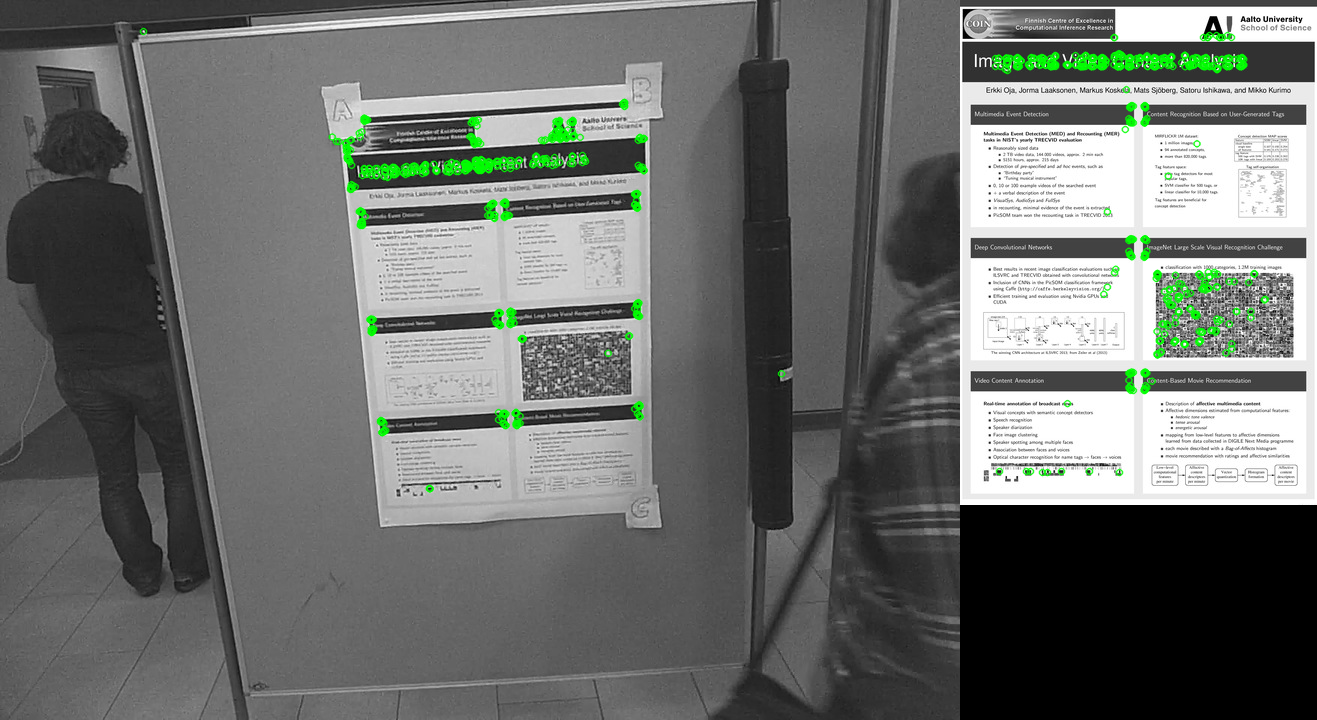
\includegraphics[scale=0.35]{keypoints_combined}
  \end{figure}
  \begin{verbatim}
      poster = cv2.imread('poster.jpeg', cv2.IMREAD_GRAYSCALE)
      frame = cv2.imread('frame.jpeg', cv2.IMREAD_GRAYSCALE)

      #Use OpenCV’s cv2.ORB_create() to create the detector and descriptor object orb
      #Apply orb.detectAndCompute() to get the keypoints and their corresponding descriptors in both images
      orb = cv2.ORB_create()
      poster_kp, poster_des = orb.detectAndCompute(poster, None)
      frame_kp, frame_des = orb.detectAndCompute(frame, None)

      #ORB returns by default 500 keypoints, which might be a good number, could be changed

      #Visualize the detections using cv2.drawKeypoints()
      poster2 = cv2.drawKeypoints(poster, poster_kp, None, color=(0, 255, 0), flags=0)
      frame2 = cv2.drawKeypoints(frame, frame_kp, None, color=(0, 255, 0), flags=0)

      poster2_resize = cv2.copyMakeBorder(poster2, 0, frame2.shape[0] - poster2.shape[0], 0, 0, cv2.BORDER_CONSTANT)
      combod = np.concatenate((frame2, poster2_resize), axis=1)
  \end{verbatim}

\subsection{One way connect}
  \begin{figure}[h]
      \centering
      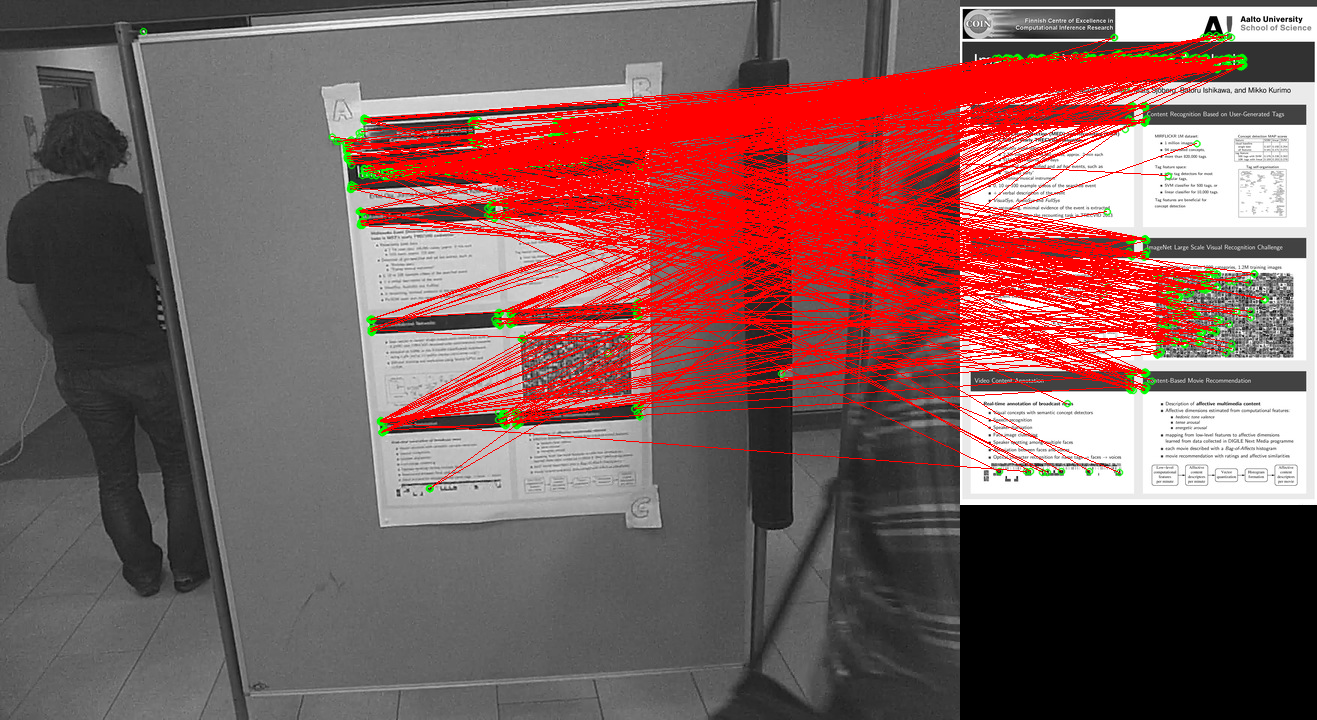
\includegraphics[scale=0.35]{one_way_match_knn}
  \end{figure}

  \begin{verbatim}
      knn = cv2.ml.KNearest_create()
      poster_des_f32 = np.asarray(poster_des, dtype=np.float32)
      frame_des_f32 = np.asarray(frame_des, dtype=np.float32)
      poster_kp_vec = cv2.KeyPoint_convert(poster_kp)
      frame_kp_vec = cv2.KeyPoint_convert(frame_kp)

      labels = np.asarray(np.arange(0, len(poster_kp)), dtype=np.float32).reshape(500, 1)
      knn.train(poster_des_f32, cv2.ml.ROW_SAMPLE, labels)
      ret, results, neighbours, dist = knn.findNearest(frame_des_f32, k=1)

      ### Connect the matching keypoint pairs across the images
      poster_offset = (frame2.shape[1], frame2.shape[0])
      red = (0, 0, 255)
      combod = np.concatenate((frame2, poster2_resize), axis=1)
      poster_resize = cv2.copyMakeBorder(poster2, 0, frame2.shape[0] - poster2.shape[0], 0, 0, cv2.BORDER_CONSTANT)

      poster_idx = 0
      for point in results:
          frame_idx = int(point[0])
          poster_kp_pos = poster_kp_vec[poster_idx]
          poster_img_pos = (int(poster_kp_pos[0] + poster_offset[0]), int(poster_kp_pos[1]))
          frame_img_pos = (int(frame_kp_vec[frame_idx][0]), int(frame_kp_vec[frame_idx][1]))
          print(poster_img_pos)
          print(frame_img_pos)
          cv2.line(combod, poster_img_pos, frame_img_pos, red, 1)
          poster_idx += 1

      #cv2.imwrite('one_way_match_knn.png', combod)
\end{verbatim}

\subsection{Two way connect}
  \begin{figure}[h]
      \centering
      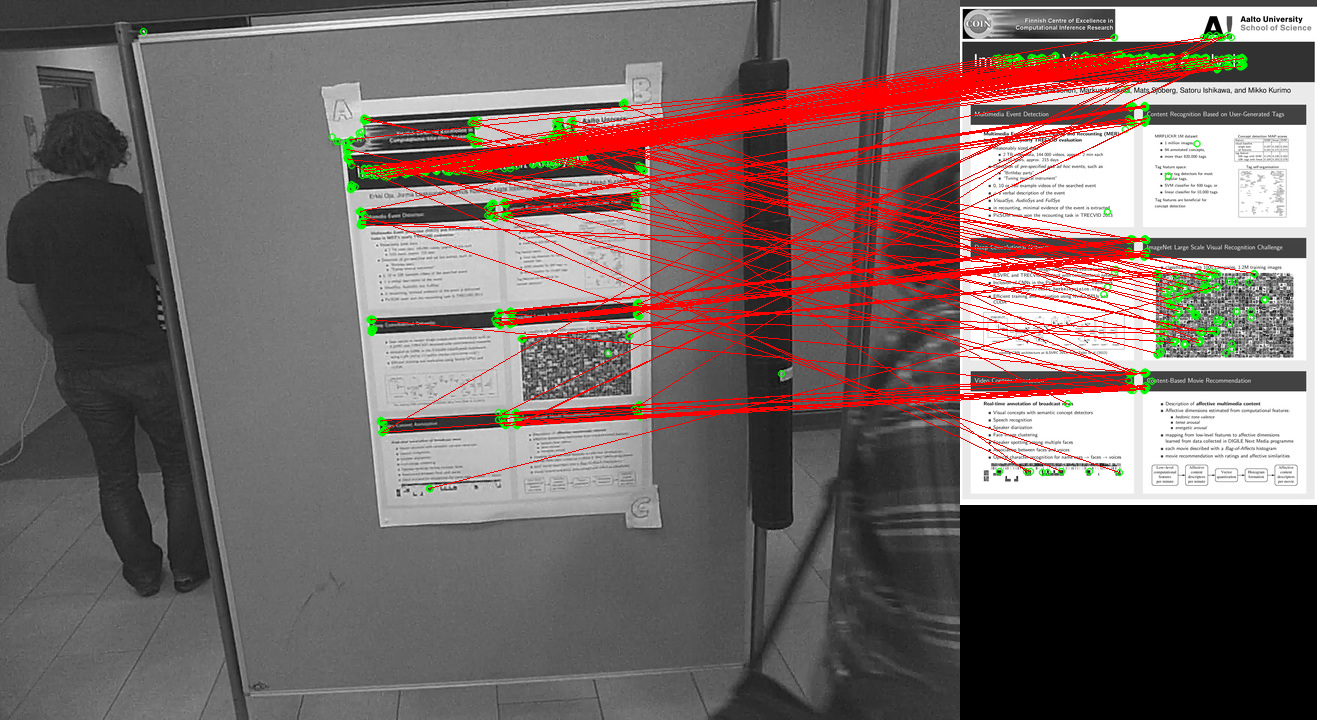
\includegraphics[scale=0.35]{two_way_match_knn}
  \end{figure}

  \begin{verbatim}
      Change to use a 1-NN matching also in the opposite direction by creating a k-NN model from the frame image’s descriptors
      Find the nearest descriptors in the first image for those in the second image, and vice versa

      If a pair of descriptors, one in the first image ant the other in the second image, are reciprocally nearest ones to each other, consider them as a matching pair

      Again connect the matching pairs and show results
      knn_ftop = cv2.ml.KNearest_create()
      knn_ftop.train(frame_des_f32, cv2.ml.ROW_SAMPLE, labels)
      ret, results_ftop, neighbours, dist = knn_ftop.findNearest(poster_des_f32, k=1)

      for frame_idx in range(len(results_ftop)):
          poster_idx = int(results_ftop[frame_idx][0])
          back_ref = int(results[poster_idx][0])
          print(frame_idx, poster_idx, back_ref)
          if frame_idx == back_ref:
              poster_kp_pos = poster_kp_vec[back_ref]
              frame_kp_pos = frame_kp_vec[poster_idx]
              poster_img_pos = (int(poster_kp_pos[0] + poster_offset[0]), int(poster_kp_pos[1]))
              frame_img_pos = (int(frame_kp_pos[0]), int(frame_kp_pos[1]))
              cv2.line(combod, poster_img_pos, frame_img_pos, red, 1)

      cv2.imwrite('two_way_match_knn.png', combod)
  \end{verbatim}

\subsection{KNN from video}
  \begin{figure}[h]
      \centering
      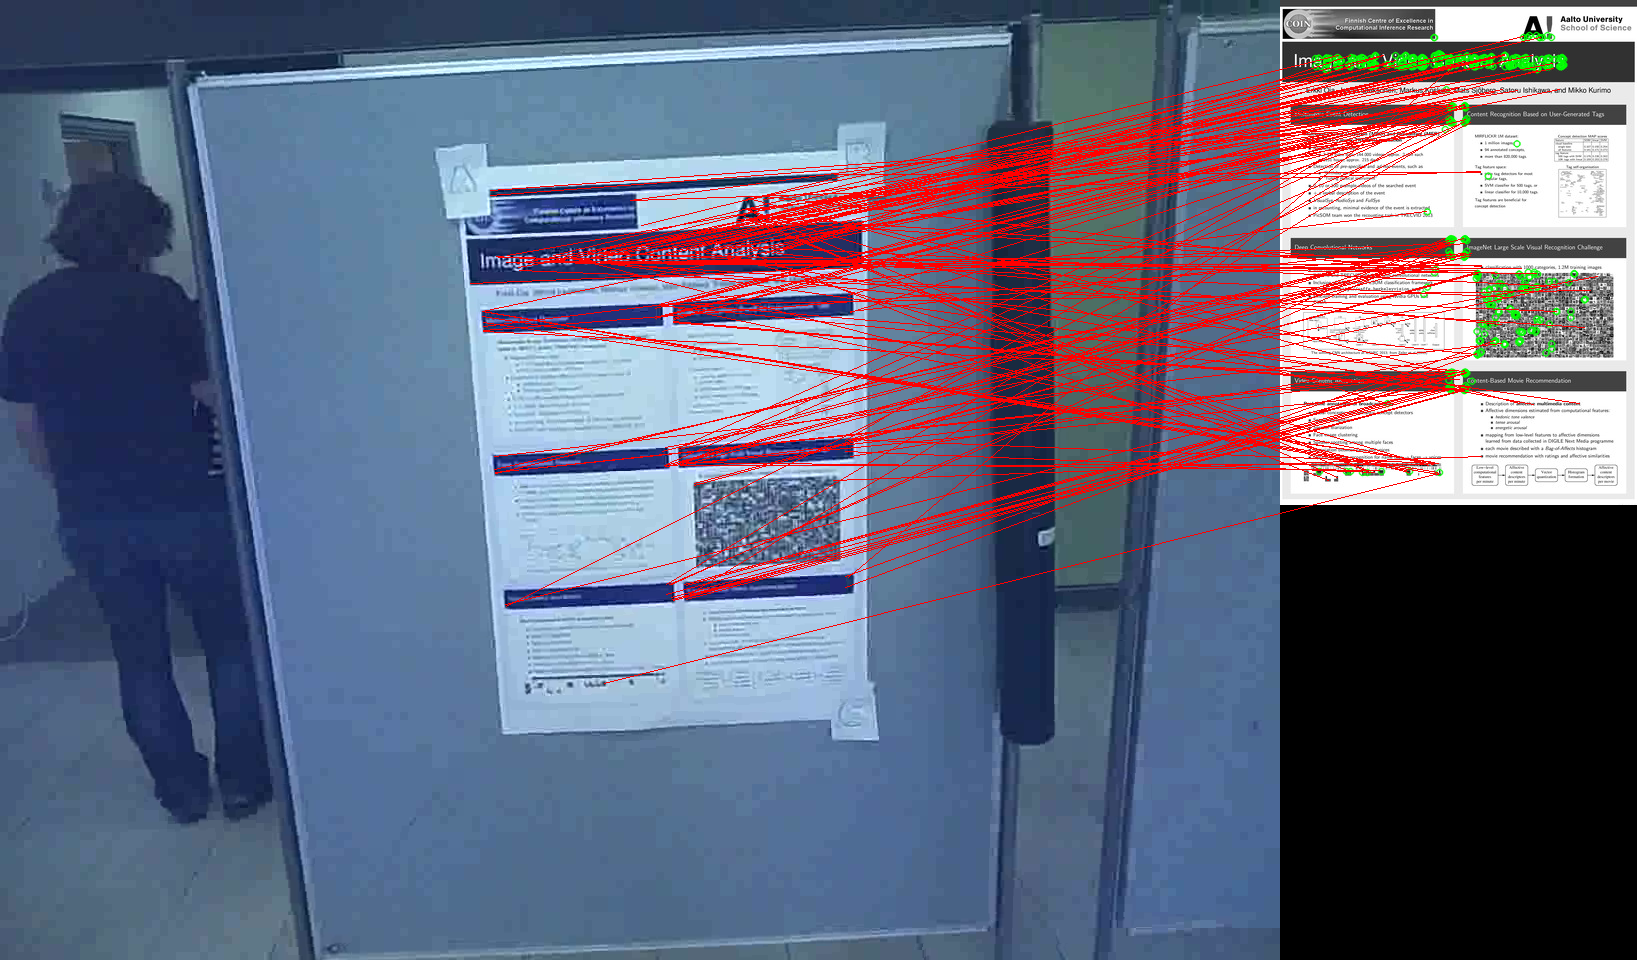
\includegraphics[scale=0.28]{knn_video}
  \end{figure}
  Example frame times:
  \begin{verbatim}
    frame processing time: 0.027774810791015625 seconds.
    frame processing time: 0.02882528305053711 seconds.
    frame processing time: 0.030350208282470703 seconds.
    frame processing time: 0.02928614616394043 seconds.
    frame processing time: 0.029371023178100586 seconds.
    frame processing time: 0.029389619827270508 seconds.
  \end{verbatim}

\subsection{Flann from video}
  \begin{figure}[h]
      \centering
      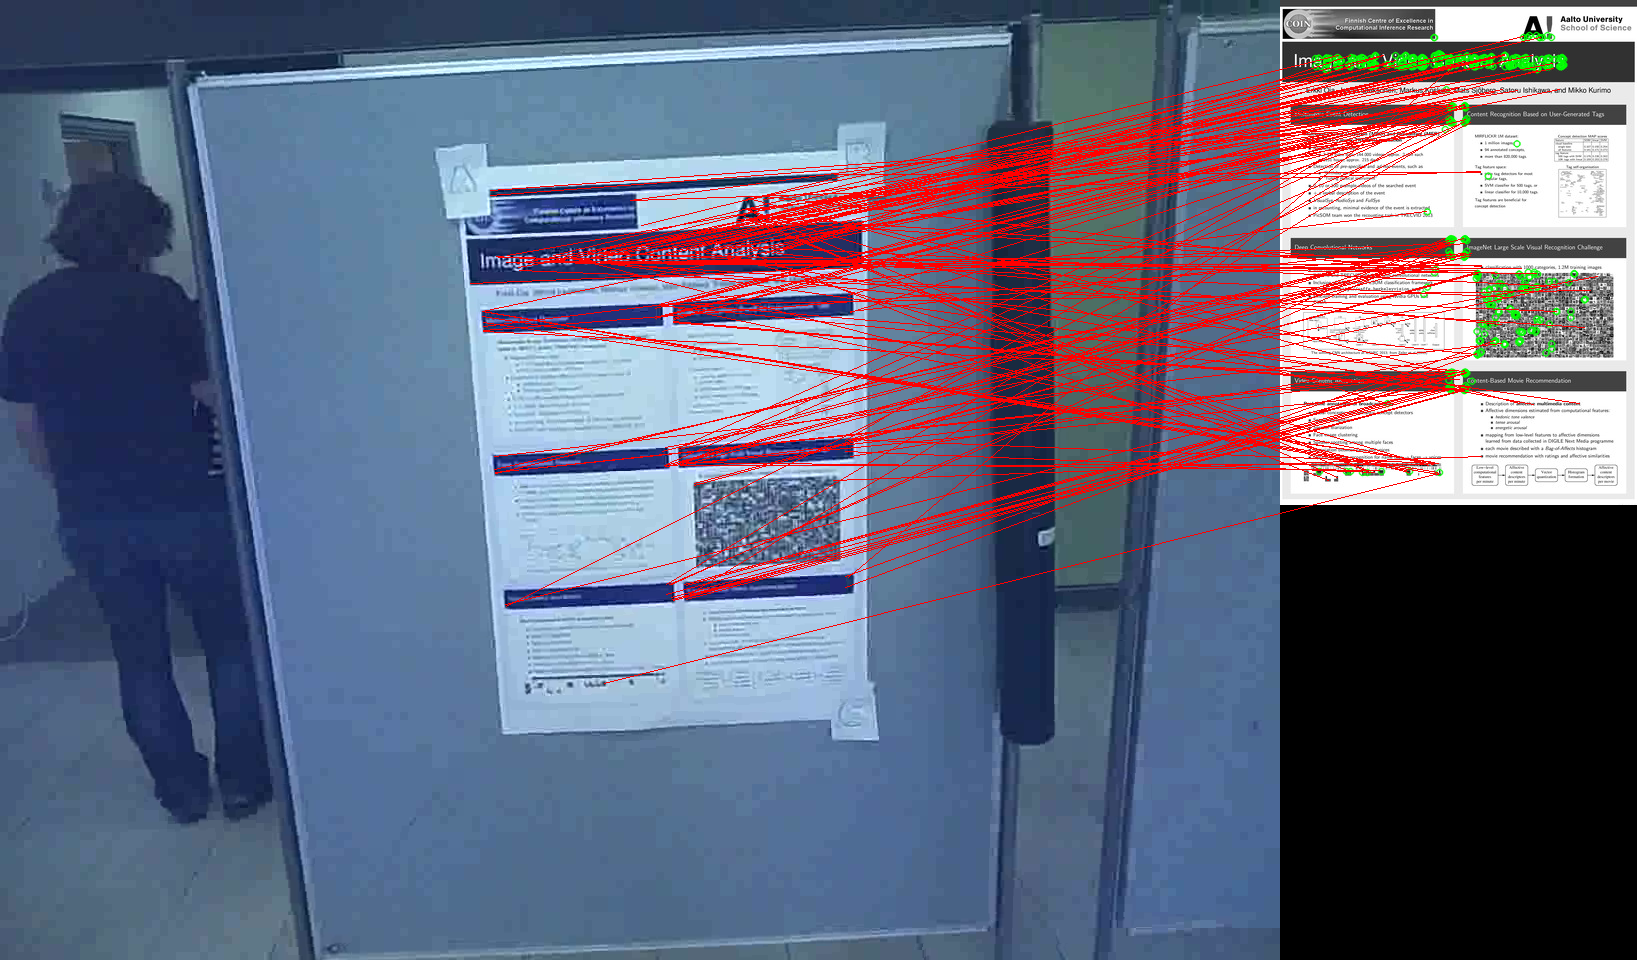
\includegraphics[scale=0.28]{flann}
  \end{figure}
  Example frame times:
  \begin{verbatim}
    frame processing time: 0.03621077537536621 seconds.
    frame processing time: 0.03606915473937988 seconds.
    frame processing time: 0.03673076629638672 seconds.
    frame processing time: 0.03754067420959473 seconds.
    frame processing time: 0.03644680976867676 seconds.
    frame processing time: 0.03664064407348633 seconds.
    frame processing time: 0.036463022232055664 seconds.
  \end{verbatim}
  Seems to be a bit slower.
  \subsection{Code for video flann and knn}
  \begin{verbatim}
      def get_neighbours_knn(train_data, test_data):
          labels = np.asarray(np.arange(0, len(train_data)), dtype=np.float32).reshape(len(train_data), 1)
          knn = cv2.ml.KNearest_create()
          knn.train(train_data, cv2.ml.ROW_SAMPLE, labels)
          ret, results, neighbours, dist = knn.findNearest(test_data, k=1)
          return results

      def get_neighbours_flann(train_data, test_data):
          FLANN_INDEX_KDTREE = 0
          index_params = dict(algorithm = FLANN_INDEX_KDTREE, trees = 5)
          search_params = dict(checks=50)   # or pass empty dictionary
          flann = cv2.FlannBasedMatcher(index_params,search_params)
          matches = flann.knnMatch(train_data, test_data, k=1)
          return matches

      def process_frame_knn(frame, poster):
          poster_offset = (frame.shape[1], frame.shape[0])
          red = (0, 0, 255)
          poster_resize = cv2.copyMakeBorder(poster, 0, frame.shape[0] - poster.shape[0], 0, 0, cv2.BORDER_CONSTANT)

          poster_kp, poster_des = orb.detectAndCompute(poster, None)
          frame_kp, frame_des = orb.detectAndCompute(frame, None)
          poster_kp_vec = cv2.KeyPoint_convert(poster_kp)
          frame_kp_vec = cv2.KeyPoint_convert(frame_kp)

          results1 = get_neighbours_knn(np.float32(poster_des), np.float32(frame_des))
          results2 = get_neighbours_knn(np.float32(frame_des), np.float32(poster_des))

          combod = np.concatenate((frame, poster_resize), axis=1)
          for frame_idx in range(len(results1)):
              poster_idx = int(results1[frame_idx][0])
              back_ref = int(results2[poster_idx][0])
              if frame_idx == back_ref:
                  poster_kp_pos = poster_kp_vec[back_ref]
                  frame_kp_pos = frame_kp_vec[poster_idx]
                  poster_img_pos = (int(poster_kp_pos[0] + poster_offset[0]), int(poster_kp_pos[1]))
                  frame_img_pos = (int(frame_kp_pos[0]), int(frame_kp_pos[1]))
                  cv2.line(combod, poster_img_pos, frame_img_pos, red, 1)

          return combod


      def process_frame_flann(frame, poster):
          poster_offset = (frame.shape[1], frame.shape[0])
          red = (0, 0, 255)
          poster_resize = cv2.copyMakeBorder(poster, 0, frame.shape[0] - poster.shape[0], 0, 0, cv2.BORDER_CONSTANT)

          poster_kp, poster_des = orb.detectAndCompute(poster, None)
          frame_kp, frame_des = orb.detectAndCompute(frame, None)
          poster_kp_vec = cv2.KeyPoint_convert(poster_kp)
          frame_kp_vec = cv2.KeyPoint_convert(frame_kp)

          results1 = get_neighbours_flann(np.float32(poster_des), np.float32(frame_des))
          results2 = get_neighbours_flann(np.float32(frame_des), np.float32(poster_des))

          combod = np.concatenate((frame, poster_resize), axis=1)
          for frame_idx in range(len(results1)):
              poster_idx = results1[frame_idx][0].trainIdx
              back_ref = results2[poster_idx][0].trainIdx
              if frame_idx == back_ref:
                  poster_kp_pos = poster_kp_vec[back_ref]
                  frame_kp_pos = frame_kp_vec[poster_idx]
                  poster_img_pos = (int(poster_kp_pos[0] + poster_offset[0]), int(poster_kp_pos[1]))
                  frame_img_pos = (int(frame_kp_pos[0]), int(frame_kp_pos[1]))
                  cv2.line(combod, poster_img_pos, frame_img_pos, red, 1)

          return combod

      cap = cv2.VideoCapture('video.avi')

      ret, frame = cap.read()
      while ret:
          start_time = time.time()
          combo_pic = process_frame_flann(frame, poster2_resize)
          #combo_pic = process_frame_knn(frame, poster2_resize)
          print('frame processing time: %s seconds.' % (time.time() - start_time))
          cv2.imwrite('knn_video.png', combo_pic)
          cv2.waitKey(1)
          ret, frame = cap.read()
  \end{verbatim}


  \section{Day 4 Homework}

\end{document}
%  LocalWords:  Jorma Laaksonen pdf py tex OpenCV libopencv dev jpg
%  LocalWords:  highgui imgproc imgcodecs greyscale png opencv ing
%  LocalWords:  texlive includegraphics Exactum Gür Ersalan
